% 2021 全国甲卷理科 19：直三棱柱与点 D、E、F
% 按固定上游 PDF 第 2 页绘制。E、F 为 AC、CC₁ 中点，D 位于棱 A₁B₁。
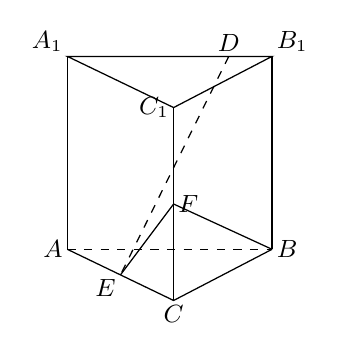
\begin{tikzpicture}[font=\small,line width=0.45pt,
  every node/.style={inner sep=1.5pt}]
  \coordinate (A1) at (0,2.8);  \coordinate (B1) at (2.6,2.8);
  \coordinate (C1) at (1.35,2.15);
  \coordinate (A) at (0,0.35); \coordinate (B) at (2.6,0.35);
  \coordinate (C) at (1.35,-0.30);
  \coordinate (D) at (2.05,2.8);
  \coordinate (E) at (0.675,0.025); \coordinate (F) at (1.35,0.925);
  % 上底、侧棱、下底（遮挡的 AB 为虚线）
  \draw (A1)--(B1)--(C1)--cycle;
  \draw (A1)--(A) (B1)--(B) (C1)--(C);
  \draw[dashed] (A)--(B);
  \draw (A)--(C)--(B);
  % 题设线段
  \draw (B)--(F) (E)--(F);
  \draw[dashed] (D)--(E);
  % 点名
  \node[anchor=south east] at (A1) {$A_1$};
  \node[anchor=south west] at (B1) {$B_1$};
  \node[anchor=east] at (C1) {$C_1$};
  \node[anchor=east] at (A) {$A$};
  \node[anchor=west] at (B) {$B$};
  \node[anchor=north] at (C) {$C$};
  \node[anchor=south] at (D) {$D$};
  \node[anchor=north east] at (E) {$E$};
  \node[anchor=west] at (F) {$F$};
\end{tikzpicture}
